% Adam report draft; prepared with AI assistance for author review.
\subsection{The US Data Show a Similar but Not Conclusive Pattern}
\label{sec:res-us}

The US results show moderate agreement with the Spanish pattern, although the evidence is not conclusive. Across ten comparable areas, Pearson correlation is $r=0.61$, with a 95\% Fisher-$z$ interval from $-0.03$ to $0.90$. Spearman correlation is also 0.61, and eight areas share the same sign. In Figure~\ref{fig:us}, Education has the highest effect in both countries: $+0.45$ Spanish grade points and $+0.43$ US GPA points. Engineering and Agriculture are below the centred reference in both. Adding area effects to university and year effects raises $R^2$ from 0.28 to 0.77 in the US and from 0.26 to 0.70 in Spain. This describes differences between aggregated cells. With only ten area pairs, the correlation remains uncertain: its interval includes zero, so the apparent agreement should be treated cautiously.

\begin{figure}[t]
  \centering
  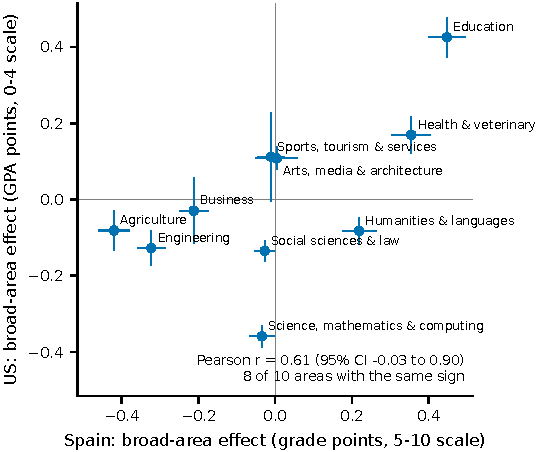
\includegraphics[width=0.92\linewidth]{fig5_us_spain}
  \caption{Fixed-effect estimates for ten common areas: Spanish graduate averages (5--10 scale) against US section GPAs (A+ = 4.3 conversion). Bars show 95\% intervals clustered by university. Pearson $r=0.61$ (95\% interval $-0.03$ to $0.90$); eight signs agree. Compare signs and ordering, not absolute magnitudes. Original figure; SIIU and Jeong et al.\ (``Course Grades'').}
  \label{fig:us}
\end{figure}

The countries do not agree in every area. Humanities and languages is above the reference in Spain ($+0.22$) but below it in the US ($-0.08$). Sports, tourism and services also changes sign, from $-0.01$ to $+0.11$, although both estimates are small. Science, mathematics and computing is close to the reference in Spain ($-0.03$) and further below it in the US ($-0.36$). These differences may partly reflect what the records measure. US departmental grades include introductory courses taken by students from other degrees, while the Spanish data describe graduates' final averages. Grouping subjects into broad areas can also hide differences within them, so we should not read every disagreement as evidence of a different grading policy.

The main result changes little across our checks. Pearson correlation is 0.62 with equal section weights across all 33 institutions, 0.61 when A+ is capped at 4.0, and 0.63 using common years. Each check keeps eight matching signs; capped-grade Spearman correlation is 0.70. Leaving out each US university keeps Pearson correlation between 0.60 and 0.63. This suggests that one institution does not drive the result, but it does not remove the uncertainty. The sensitivity runs use conventional coefficient errors, whereas Figure~\ref{fig:us} uses university-clustered intervals. The small number of areas and different grade definitions remain limitations.
